% Provenance (never printed): old seconde/premiere S material on the ocean
% (the ocean as a layered fluid, its heat, upwelling and productive waters);
% see sources/book2/PROVENANCE.md. All profiles are WOA23 columns, all
% densities the EOS-80 one-atmosphere equation, computed in
% figdata/grade-10/ocean_profiles.py.
\chapter{分层的海洋}\label{ch:g10:layered-ocean}

夏日里，你从海滩游出，进入温暖宜人的海水中。
接着你把腿垂下去——脚却碰到了突然变冷的水，
离水面仅几米深。海水并不是上下均匀混合的，
而是由一层层水体组成：上层温暖、较轻，下层寒冷、较重。
在广阔的大洋中，这种分层可延伸至数千米深，
它决定了海洋在哪里是沙漠，在哪里生机勃勃。本章
深入探讨海洋的内部：海洋如何测量，温度和盐度如何随深度变化，
各层为何稳定，
以及寒冷的深层水在何处重新升回表层。

\begin{recall}
海水含有溶解的盐类：其盐度平均约为每千克海水含 \num{35}~克盐，
且因海域而异。风驱动表层洋流和大型环流；
深层冷而咸的水沿海底缓慢流动（第 1 册，八年级）。
密度等于质量除以体积（物理分册）。
浮游植物是微小的藻类，需要光和矿物营养盐，
通过光合作用生长，并为海洋的其他食物链提供食物
（生物分册）。
\end{recall}

\section{测量海洋}

海洋面积约为 3.62 亿~\unit{km^2}，平均深度为
\qty{3682}{m}，总水量约为 \num{1.33}~十亿~\unit{km^3}。
海水大部分位于光无法到达的深处，
只能通过向下投放仪器进行测量。
% ledger: charette:ocean-volume

海洋学家从船上用缆绳放下一个框架，框架上装有传感器，
用于测量海水的电导率（由此计算盐度）、
温度和压强（由此得出深度）；框架周围环绕着一圈采水瓶，
可在选定深度关闭，以便将水样带回船上。
自 2000 年以来，一支由自动浮标组成的船队已积累了数百万条剖面数据。
每个浮标随洋流漂移，位于 \qty{1000}{m} 深处，
大约每十天下沉至 \qty{2000}{m}，
然后在上升至水面的过程中测量温度和盐度，
并通过卫星发送其剖面数据。
% ledger: argo:fleet

\begin{dated}{2026}
国际 Argo 阵列拥有接近 4000 个在用浮标；
其第三百万条剖面数据采集于 2024 年 7 月。
% ledger: argo:fleet
\end{dated}

\begin{omfigure}
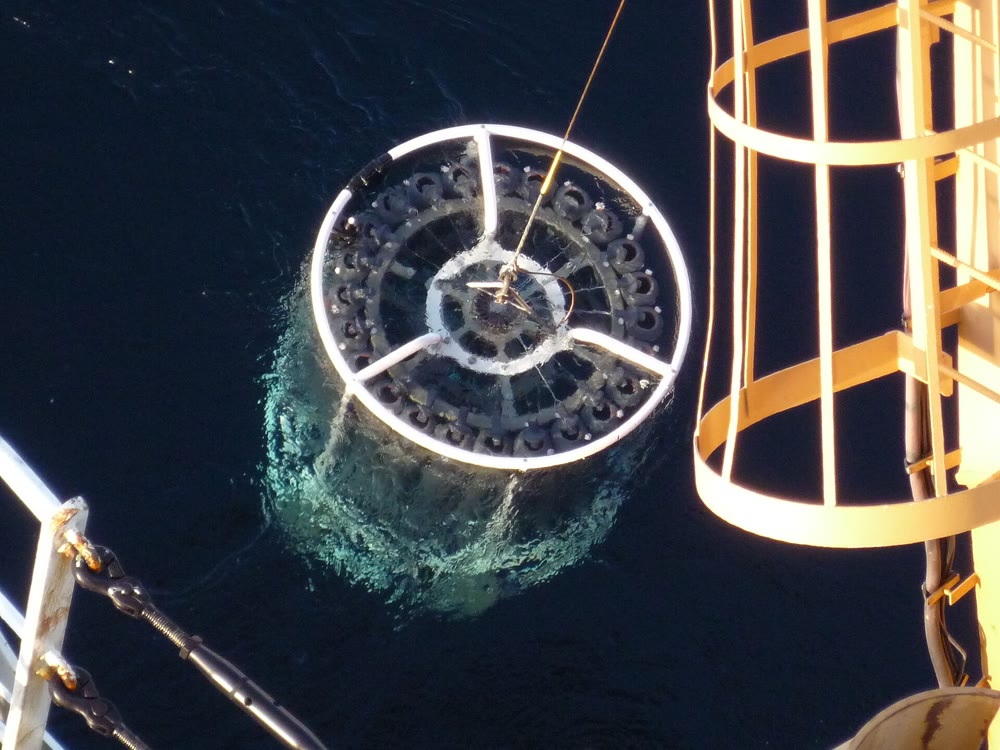
\includegraphics[height=4.4cm]{images/book2/g10-noaa-ctd-rosette.jpg}\hspace{0.4cm}%
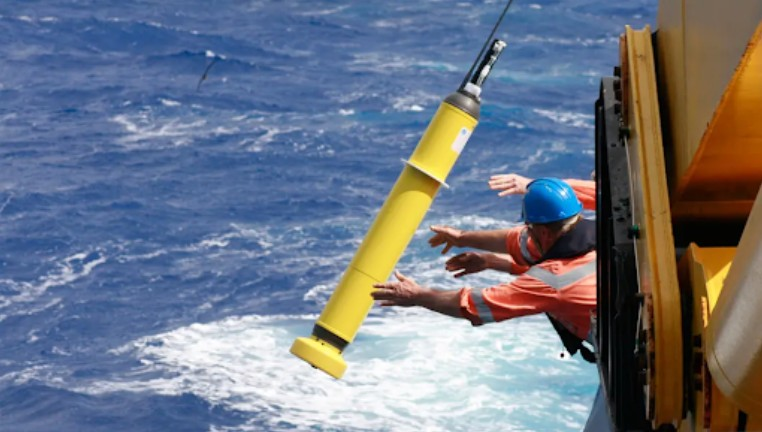
\includegraphics[height=4.4cm]{images/book2/g10-noaa-argo-float.jpg}

{\small 左：围绕传感器的采水瓶组，2008 年在北极科考船旁
被拉回水面（照片：Pablo Clemente-Colon，
NOAA Photo Library）。右：一个剖面浮标正从科考船上释放
（照片：NOAA Global Ocean Monitoring and Observing
Program）。两者均为公有领域。}
\end{omfigure}

对数十年的测量结果取平均，可得到海洋随深度变化的图景。
本章的剖面即为此类平均值，取自
\emph{World Ocean Atlas 2023}，由美国国家海洋和大气管理局（NOAA）的
国家环境信息中心发布。

\section{温度随深度的变化}

\begin{omfigure}
\begin{tikzpicture}
\begin{axis}[omrecord, omdepth, width=0.62\linewidth, height=8.2cm,
  axis x line=top, xmin=-3, xmax=31, ymin=0, ymax=2000,
  xlabel={温度（\unit{\degreeCelsius}）}, ylabel={深度（\unit{m}）},
  tick label style={font=\small}, label style={font=\small},
  legend style={font=\scriptsize, at={(0.98,0.03)}, anchor=south east}]
\addplot[omThm!85!black, thick] table[x=t, y=depth] {figdata/out/grade-10-ocean_profiles-site-warmpool.dat};
\addplot[omDef!85!black, thick] table[x=t, y=depth] {figdata/out/grade-10-ocean_profiles-site-atlantic.dat};
\addplot[black!70, thick, dashed] table[x=t, y=depth] {figdata/out/grade-10-ocean_profiles-site-arctic.dat};
\legend{{热带太平洋，北纬 5.5\textdegree}, {北大西洋，北纬 40.5\textdegree}, {北冰洋，北纬 75.5\textdegree}}
\node[font=\scriptsize, anchor=west] (ml) at (axis cs:21,430) {混合层};
\draw[black!50] (ml.north east) -- (axis cs:28.9,35);
\node[font=\scriptsize, anchor=west] (tc) at (axis cs:15.5,600) {温跃层};
\draw[black!50] (tc.north) -- (axis cs:19.9,150);
\node[font=\scriptsize, anchor=west] at (axis cs:7,1500) {深海};
\end{axis}
\end{tikzpicture}

{\small 三个地点的平均温度随深度的变化（深度向下增加）。
数据：World Ocean Atlas 2023，年平均值，NOAA NCEI。}
\end{omfigure}
% ledger: data:b2-woa23 (profiles in figdata/grade-10/ocean_profiles.py)

阳光从上方加热海洋表层。风和浪将这层温暖的水搅动成
温度近乎均匀的一层。其下，温度在
几百米内迅速下降；再往深处，温度缓慢下降，直至
达到充满大洋盆地的寒冷的水。

\begin{definition}[混合层]\label{def:g10:layered-ocean:mixed-layer}
海洋的\emph{混合层}\index{混合层}是表层海水，
受风和浪搅动，其中温度和盐度
几乎不随深度变化。
\end{definition}

\begin{definition}[温跃层；盐跃层；密度跃层；深海]\label{def:g10:layered-ocean:thermocline}
\emph{温跃层}\index{温跃层}是位于\omterm{def:g10:layered-ocean:mixed-layer}{混合层}之下的一层，
其中温度随深度迅速下降。
盐度随深度迅速变化的一层称为\emph{盐跃层}\index{盐跃层}；
密度随深度迅速增大的一层称为
\emph{密度跃层}\index{密度跃层}。在它们之下是\emph{深海
}\index{深海}，水温寒冷，变化缓慢。
\end{definition}

在热带太平洋，\omterm{def:g10:layered-ocean:mixed-layer}{混合层}温度为 \qty{29.2}{\degreeCelsius}，
厚约 \qty{60}{m}；在 \qty{70}{m} 至 \qty{300}{m} 之间，温度
下降近十九度，在 \qty{1000}{m} 处降至 \qty{4.5}{\degreeCelsius}。
在北大西洋，表层较凉，
降温更为平缓。在北冰洋，整个水柱都保持在
\qty{0}{\degreeCelsius} 上下两度之内，没有
值得一提的温暖表层。
% ledger: data:b2-woa23

\begin{method}[读懂海洋剖面]\label{met:g10:layered-ocean:profile}
\begin{enumerate}
  \item 认清坐标轴：深度向下增加，
        被测量沿顶部读取。
  \item \omterm{def:g10:layered-ocean:mixed-layer}{混合层}是曲线近乎竖直的上部，
        其深度是曲线开始偏离竖直的位置（一个常用
        规则：温度比表层值下降 \qty{0.5}{\degreeCelsius}
        时的深度）。
  \item \omterm{def:g10:layered-ocean:thermocline}{温跃层}是曲线最接近水平的部分：
        在最小的深度范围内温度变化最大。
  \item 在其下方读取深层数值，并比较同一深度的不同站点。
\end{enumerate}
\end{method}

\omterm{def:g10:layered-ocean:mixed-layer}{混合层}随季节变化。冬季，表层失去热量，
风暴搅动海水，\omterm{def:g10:layered-ocean:mixed-layer}{混合层}加深；夏季，太阳加热
一层较薄的表层水，较弱的风无法将其向下混合，于是
近表层形成\emph{季节性\omterm{def:g10:layered-ocean:thermocline}{温跃层}}——即
游泳者双脚触到的冷水。

\begin{omfigure}
\begin{tikzpicture}
\begin{axis}[omrecord, omdepth, width=0.6\linewidth, height=6.6cm,
  axis x line=top, xmin=12, xmax=24, ymin=0, ymax=300,
  xlabel={温度（\unit{\degreeCelsius}）}, ylabel={深度（\unit{m}）},
  tick label style={font=\small}, label style={font=\small},
  legend style={font=\scriptsize, at={(0.98,0.03)}, anchor=south east}]
\addplot[omDef!85!black, thick] table[x=t_feb, y=depth] {figdata/out/grade-10-ocean_profiles-season.dat};
\addplot[omThm!85!black, thick] table[x=t_aug, y=depth] {figdata/out/grade-10-ocean_profiles-season.dat};
\legend{二月, 八月}
\end{axis}
\end{tikzpicture}

{\small 北大西洋的冬季与夏季（40.5\textdegree N，
30.5\textdegree W）。月平均温度，分别为二月与八月。
二月时\omterm{def:g10:layered-ocean:mixed-layer}{混合层}深约 \qty{170}{m}；八月时，
厚约 \qty{15}{m} 的暖层位于季节性\omterm{def:g10:layered-ocean:thermocline}{温跃层}之上。数据来源：World
Ocean Atlas 2023, NOAA NCEI。}
\end{omfigure}
% ledger: data:b2-woa23 (mixed-layer depths by the 0.5 degC rule, computed in figdata/grade-10/ocean_profiles.py)

\section{盐度与密度}

海水的密度取决于其温度和盐度。它
由一个国际公认的公式计算得出，即海水状态方程，
该公式拟合了实验室测量数据。

\begin{proposition}[海水的密度]\label{prop:g10:layered-ocean:density}
海水的密度随盐度增大而增大，随温度
升高而减小。在表层压强下，盐度为 35 的海水
在 \qty{0}{\degreeCelsius} 时密度为 \qty{1028.1}{kg/m^3}，
在 \qty{25}{\degreeCelsius} 时为 \qty{1023.3}{kg/m^3}；纯水在
\qty{4}{\degreeCelsius} 时密度为 \qty{1000.0}{kg/m^3}。
\end{proposition}
% ledger: unesco:eos80 (values computed in figdata/grade-10/ocean_profiles.py)

\begin{omfigure}
\begin{tikzpicture}
\begin{axis}[omrecord, width=0.7\linewidth, height=6.2cm, xmin=-2, xmax=30,
  ymin=1016, ymax=1033, xlabel={温度（\unit{\degreeCelsius}）},
  ylabel={密度（\unit{kg/m^3}）}, tick label style={font=\small},
  label style={font=\small}, yticklabel style={/pgf/number format/1000 sep={}}]
\addplot[omThm!85!black, thick] table[x=t, y=rho_s38] {figdata/out/grade-10-ocean_profiles-eos.dat};
\addplot[black!80, thick] table[x=t, y=rho_s35] {figdata/out/grade-10-ocean_profiles-eos.dat};
\addplot[omDef!85!black, thick] table[x=t, y=rho_s30] {figdata/out/grade-10-ocean_profiles-eos.dat};
\node[font=\scriptsize, anchor=south west, omThm!85!black] at (axis cs:1,1030.75) {盐度 38};
\node[font=\scriptsize, anchor=south west] at (axis cs:1,1028.35) {盐度 35};
\node[font=\scriptsize, anchor=south west, omDef!85!black] at (axis cs:1,1024.35) {盐度 30};
\end{axis}
\end{tikzpicture}

{\small 表层压强下海水的密度随其
温度的变化，对应三种盐度（依据国际
海水状态方程计算）。}
\end{omfigure}
% ledger: unesco:eos80

图中可见两点。盐度每增加一个单位，密度约增加
\qty{0.8}{kg/m^3}。温度每升高一度，在 \qty{25}{\degreeCelsius} 时密度约减少 \qty{0.31}{kg/m^3}，
在 \qty{10}{\degreeCelsius} 时约减少 \qty{0.18}{kg/m^3}，
而在 \qty{0}{\degreeCelsius} 附近仅约减少 \qty{0.06}{kg/m^3}：在温暖的海域，温度决定密度，
在寒冷海域，起决定作用的则是盐度。
% ledger: unesco:eos80 (slopes computed in figdata/grade-10/ocean_profiles.py)

\begin{remark}
本章的密度均按表层压强计算。
上方海水的压力使海水略有压缩，约为每千米深度
\qty{4}{kg/m^3}；海洋学家在相同压强下比较水团，
从而只需考虑温度与盐度。
\end{remark}
% ledger: unesco:eos80-checks (computed in figdata/grade-10/ocean_profiles.py: 3.9 kg/m3 per km from the 10000-dbar check values)

\begin{omfigure}
\begin{tikzpicture}
\begin{axis}[name=sal, omrecord, omdepth, width=0.5\linewidth, height=7.2cm,
  axis x line=top, xmin=27.5, xmax=37, ymin=0, ymax=1000,
  xlabel={盐度}, ylabel={深度（\unit{m}）},
  tick label style={font=\small}, label style={font=\small}]
\addplot[omThm!85!black, thick] table[x=s, y=depth] {figdata/out/grade-10-ocean_profiles-site-warmpool.dat};
\addplot[omDef!85!black, thick] table[x=s, y=depth] {figdata/out/grade-10-ocean_profiles-site-atlantic.dat};
\addplot[black!70, thick, dashed] table[x=s, y=depth] {figdata/out/grade-10-ocean_profiles-site-arctic.dat};
\node[font=\scriptsize, anchor=west, align=left] at (axis cs:28.2,120) {北冰洋 \\盐跃层};
\end{axis}
\begin{axis}[at={(sal.east)}, anchor=west, xshift=0.9cm, omrecord, omdepth,
  width=0.5\linewidth, height=7.2cm, axis x line=top, xmin=1021, xmax=1028.5, yticklabels={},
  ymin=0, ymax=1000, xlabel={密度（\unit{kg/m^3}）},
  tick label style={font=\small}, label style={font=\small},
  xticklabel style={/pgf/number format/1000 sep={}},
  legend style={font=\scriptsize, at={(0.03,0.03)}, anchor=south west}]
\addplot[omThm!85!black, thick] table[x=rho, y=depth] {figdata/out/grade-10-ocean_profiles-site-warmpool.dat};
\addplot[omDef!85!black, thick] table[x=rho, y=depth] {figdata/out/grade-10-ocean_profiles-site-atlantic.dat};
\addplot[black!70, thick, dashed] table[x=rho, y=depth] {figdata/out/grade-10-ocean_profiles-site-arctic.dat};
\legend{热带太平洋, 北大西洋, 北冰洋}
\end{axis}
\end{tikzpicture}

{\small 盐度（左）与表层压强下的密度（右）随深度的变化，
取自温度剖面的三个站点。各站点的密度均随深度增大。
数据：World Ocean Atlas 2023，NOAA NCEI；
密度由海水国际状态方程计算。}
\end{omfigure}
% ledger: data:b2-woa23, unesco:eos80

在热带太平洋，\omterm{def:g10:layered-ocean:thermocline}{密度跃层}与\omterm{def:g10:layered-ocean:thermocline}{温跃层}重合。在北冰洋，
温度几乎不变，但盐度由表层的 28（因河流与冰融而变淡）
增至 \qty{500}{m} 深处的 34.8，\omterm{def:g10:layered-ocean:thermocline}{盐跃层}即为\omterm{def:g10:layered-ocean:thermocline}{密度跃层}。
各情形中，密度
均随深度增大。
% ledger: data:b2-woa23

\begin{definition}[层结]\label{def:g10:layered-ocean:stratification}
海水密度随深度增大时，海洋具有\emph{层结}\index{层结}：
轻水位于重水之上，水体成层分布。
\end{definition}

\omterm{def:g10:layered-ocean:stratification}{层结}的海洋是稳定的。一团水被压入较重的水中，
它比周围的水轻，会浮回原处；被推向上方的一团水则会沉回原处。
要使各层混合，风须克服这一作用；\omterm{def:g10:layered-ocean:thermocline}{密度跃层}越强，
混合就越难：\omterm{def:g10:layered-ocean:thermocline}{温跃层}是一层盖子，将表层与\omterm{def:g10:layered-ocean:thermocline}{深海}隔开。
\omterm{def:g10:layered-ocean:thermocline}{深海}中充满了很久以前沉下的水，它们来自寒冷的极地海域，
那里的表层水变得足够致密，
因而下沉（见第 1 册，八年级）。

\section{上升流}

\begin{definition}[上升流]\label{def:g10:layered-ocean:upwelling}
\emph{上升流}\index{上升流}是指冷水从表层之下
向上涌升，以补充被风推离的表层水。它发生在
某些海岸沿岸及开阔海洋中。
\end{definition}
% ledger: noaa:upwelling

沿海岸，与海岸平行吹的风拖动表层水；
由于地球自转，海水并不简单地随风流动，而是
偏离风向：在北半球向右偏，
在南半球向左偏（其原理属于
大学阶段的内容）。在秘鲁近海，风沿海岸
向赤道吹，表层水被推向外海；冷水在
海岸附近上升以补充。\omterm{def:g10:layered-ocean:upwelling}{上升流}也发生在赤道沿线，
信风将赤道两侧的表层水推离赤道。
% ledger: noaa:upwelling, kessler:peru-upwelling

\begin{omfigure}
\begin{tikzpicture}[font=\footnotesize, >={Stealth[length=2mm]}]
  % ocean and thermocline
  \fill[omDef!12] (0,-3.2) rectangle (8.2,0);
  \fill[omDef!30] (0,-3.2) -- (0,-2.0) .. controls (3,-2.0) and (5.5,-1.6) .. (7.4,-0.35) -- (8.2,0) -- (8.2,-3.2) -- cycle;
  \draw[omDef!80!black, dashed] (0,-2.0) .. controls (3,-2.0) and (5.5,-1.6) .. (7.4,-0.35);
  \node[anchor=north west, omDef!80!black] at (0.1,-2.05) {温跃层};
  \node[anchor=west, black!70] at (0.15,-0.9) {温暖表层水};
  \node[anchor=west, black!70] at (0.15,-2.75) {寒冷、富含营养物质的水};
  % land
  \fill[omExo!30, draw=black!60] (7.0,-3.2) -- (8.2,-0.1) -- (8.6,0.0) -- (9.6,1.2) -- (10.6,2.2) -- (10.6,-3.2) -- cycle;
  \node[anchor=south, align=center] at (9.9,-1.6) {陆地};
  % surface flow and rising water
  \draw[->, thick, omThm!80!black] (7.2,-0.3) -- (3.6,-0.3);
  \node[anchor=south, omThm!80!black] at (5.4,-0.25) {表层水被推向外海};
  \foreach \x/\y in {6.1/-2.1, 6.8/-1.7} \draw[->, thick, omDef!80!black] (\x,\y) -- (\x+0.45,\y+1.15);
  \node[anchor=north, omDef!80!black, align=center] at (6.0,-2.25) {冷水上升};
  % wind along the shore, northward: with west on the left and east on the
  % right the reader looks north, so the wind goes into the page
  \draw[black!70, thick] (2.6,1.0) circle (0.22);
  \draw[black!70, thick] (2.6,1.0) ++(45:0.22) -- ++(225:0.44) (2.6,1.0) ++(135:0.22) -- ++(315:0.44);
  \node[anchor=west, align=left] at (2.9,1.0) {风沿海岸吹向赤道 \\（向北，指向纸面内）};
  \node[anchor=north west, black!60] at (0,-3.25) {$\leftarrow$ 西};
  \node[anchor=north east, black!60] at (10.6,-3.25) {东 $\rightarrow$};
\end{tikzpicture}

{\small 秘鲁近海的沿岸\omterm{def:g10:layered-ocean:upwelling}{上升流}（由西向东的示意剖面，
不按比例）：风沿海岸向赤道吹，
即向北、指向纸面内；表层水向其左侧偏转并被推向外海；
冷水从\omterm{def:g10:layered-ocean:thermocline}{温跃层}之下在海岸附近上升以补充。}
\end{omfigure}

上升的水不仅冷。在受阳光照射的表层之下，
沉降并分解的死亡浮游生物残骸释放出矿物营养物质，
这些正是浮游植物所需的。被带回光照层后，这些营养物质
使\omterm{def:g10:layered-ocean:upwelling}{上升流}区成为海洋中生产力最高的水域，并拥有
最丰富的渔场。在海洋\omterm{def:g10:layered-ocean:stratification}{层结}强而无水体将深层水带上来之处，
受光层的营养物质耗尽：亚热带环流的中心
即海洋中的沙漠。
% ledger: noaa:upwelling

\begin{omfigure}
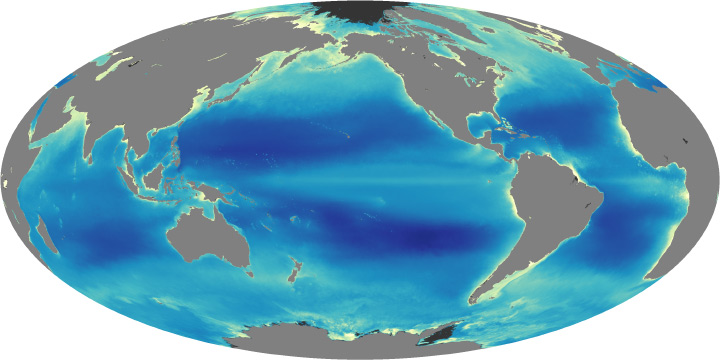
\includegraphics[width=0.8\linewidth]{images/book2/g10-nasa-ocean-chlorophyll.jpg}

{\small 从太空观测的浮游植物叶绿素（2002--2010 年平均），
由深蓝（极少）经浅蓝至黄色（很多）；
陆地为灰色。秘鲁海岸及太平洋赤道沿线的
条带十分醒目；环流区呈深蓝色。图像：Jesse Allen 与 Robert
Simmon，NASA Earth Observatory（公有领域）。}
\end{omfigure}

\begin{omfigure}
\begin{tikzpicture}
\begin{axis}[omrecord, omdepth, width=0.6\linewidth, height=7.2cm,
  axis x line=top, xmin=4, xmax=26, ymin=0, ymax=600,
  xlabel={温度（\unit{\degreeCelsius}）}, ylabel={深度（\unit{m}）},
  tick label style={font=\small}, label style={font=\small},
  legend style={font=\scriptsize, at={(0.98,0.03)}, anchor=south east}]
\addplot[omExo!85!black, thick] table[x=t, y=depth] {figdata/out/grade-10-ocean_profiles-site-peru.dat};
\addplot[omThm!85!black, thick] table[x=t, y=depth] {figdata/out/grade-10-ocean_profiles-site-gyre.dat};
\addplot[black!40, dashed, domain=0:600, samples=2] ({15}, {x});
\legend{{秘鲁近海，13.5\textdegree S}, {南太平洋环流，20.5\textdegree S}}
\end{axis}
\end{tikzpicture}

{\small 秘鲁近海处，冷水靠近海面：温度为
\qty{15}{\degreeCelsius}（虚线）的水位于约 \qty{65}{m} 深处，
而在离赤道较远的南太平洋环流中心，该水层
接近 \qty{300}{m} 深。数据：World Ocean Atlas 2023，年平均值，
NOAA NCEI。}
\end{omfigure}
% ledger: data:b2-woa23

\section{练习}

\begin{exercise}[$\star$]\label{exo:g10:layered-ocean:1}
定义\omterm{def:g10:layered-ocean:mixed-layer}{混合层}和\omterm{def:g10:layered-ocean:thermocline}{温跃层}。是什么搅动了\omterm{def:g10:layered-ocean:mixed-layer}{混合层}？
\end{exercise}

\begin{exercise}[$\star$]\label{exo:g10:layered-ocean:2}
定义\omterm{def:g10:layered-ocean:upwelling}{上升流}。为什么\omterm{def:g10:layered-ocean:upwelling}{上升流}海域的海水生物资源丰富？
\end{exercise}

\begin{exercise}[$\star$]\label{exo:g10:layered-ocean:3}
利用三个站点的温度剖面，
分别给出热带太平洋和北冰洋的海面温度，
以及 \qty{1000}{m} 深处的温度。
\end{exercise}

\begin{exercise}[$\star$]\label{exo:g10:layered-ocean:4}
哪种情况下盐度为 35 的海水密度更大：温度为 \qty{25}{\degreeCelsius}
还是 \qty{0}{\degreeCelsius}？在相同温度下，盐度为 35 的海水与纯水相比，
哪一个密度更大？请利用本章中的数值。
\end{exercise}

\begin{exercise}[$\star$]\label{exo:g10:layered-ocean:5}
说明剖面浮标如何测量海洋的剖面，
以及为何在船只很少到达的海域，浮标尤为有用。
\end{exercise}

\begin{exercise}[$\star\star$]\label{exo:g10:layered-ocean:6}
海洋面积为 3.6184 亿~\unit{km^2}，平均深度为
\qty{3682}{m}。试以立方千米为单位计算其体积；
顶部 \qty{100}{m} 占其深度的几分之几？
\end{exercise}

\begin{exercise}[$\star\star$]\label{exo:g10:layered-ocean:7}
在八月北大西洋的剖面中，海面温度为
\qty{22.7}{\degreeCelsius}，\qty{15}{m} 处为 \qty{22.2}{\degreeCelsius}，
\qty{20}{m} 处为 \qty{21.8}{\degreeCelsius}，\qty{50}{m} 处为 \qty{17.3}{\degreeCelsius}。
利用方法中的规则，估算\omterm{def:g10:layered-ocean:mixed-layer}{混合层}的深度。
\qty{20}{m} 至 \qty{50}{m} 之间的温度平均下降速率是多少，
即每米下降多少度？
\end{exercise}

\begin{exercise}[$\star\star$]\label{exo:g10:layered-ocean:8}
同一北大西洋站点，海面温度二月为 \qty{15.3}{\degreeCelsius}，
八月为 \qty{22.7}{\degreeCelsius}；而在 \qty{300}{m} 深处，
两个月温度均为 \qty{13.5}{\degreeCelsius}。试说明深层水
为何不随季节变化，以及冬季\omterm{def:g10:layered-ocean:mixed-layer}{混合层}为何
远比夏季的\omterm{def:g10:layered-ocean:mixed-layer}{混合层}深。
\end{exercise}

\begin{exercise}[$\star\star$]\label{exo:g10:layered-ocean:9}
在 \qty{10}{\degreeCelsius} 附近，盐度每增加一个单位，密度增加
\qty{0.78}{kg/m^3}，而升温一度使密度减少 \qty{0.18}{kg/m^3}。
需要升温多少度，才能抵消一个单位盐度的效应？
在 \qty{0}{\degreeCelsius} 附近，同样的问题请再作答，此处升温一度
只使密度减少 \qty{0.06}{kg/m^3}。对极地海域，
你能得出什么结论？
\end{exercise}

\begin{exercise}[$\star\star$]\label{exo:g10:layered-ocean:10}
在北冰洋，表层水温为 \qty{-1.4}{\degreeCelsius}，
盐度为 28.1；在 \qty{200}{m} 深处，温度同为 \qty{-1.4}{\degreeCelsius}，
盐度为 33.3。两处的密度分别为 \qty{1022.6}{kg/m^3} 和
\qty{1026.8}{kg/m^3}。是什么使深层水的密度更大？请说出两者
之间那一层的名称。
\end{exercise}

\begin{exercise}[$\star\star$]\label{exo:g10:layered-ocean:11}
说明\omterm{def:g10:layered-ocean:stratification}{层结}的海洋为何稳定，并以一团表层海水
被波浪压入深处为例加以说明。
\end{exercise}

\begin{exercise}[$\star\star\star$]\label{exo:g10:layered-ocean:12}
盐度为 35 的海水一升，温度由 \qty{0}{\degreeCelsius} 升至
\qty{25}{\degreeCelsius}。利用本章的密度数值，计算其质量，再计算其新体积。
此时它膨胀了多少毫升？一层厚 \qty{700}{m} 的海洋
若以相同比例升温，其厚度增长多少？
（这是对真实海洋升温的大幅夸大，
仅用于说明这一效应。）
\end{exercise}

\begin{exercise}[$\star\star\star$]\label{exo:g10:layered-ocean:13}
在热带太平洋，\qty{50}{m} 处的密度为 \qty{1021.6}{kg/m^3}，
\qty{200}{m} 处为 \qty{1026.0}{kg/m^3}；在二月的北大西洋，
表层 \qty{150}{m} 内的温度几乎不变。两者之中，
哪一处的风暴更容易把水搅动至 \qty{150}{m} 深处？请说明理由。
\end{exercise}

\begin{exercise}[$\star\star\star$]\label{exo:g10:layered-ocean:14}
在叶绿素图上，找出远离任何海岸的开阔海洋中的两个高叶绿素区域，
以及一个面积很大的极低叶绿素区域。
利用本章内容，逐一解释。
\end{exercise}

\begin{exercise}[$\star\star\star$]\label{exo:g10:layered-ocean:15}
设某剖面浮标从 \qty{1000}{m} 下沉至 \qty{2000}{m}，用时六小时，
随后用十小时上浮至海面。求其在各阶段的平均竖直速度，
单位为厘米每秒。若其上浮时每 \qty{2}{s} 测量一次，
一条剖面共包含多少次测量，
相邻两次测量之间的平均深度间隔是多少？
\end{exercise}

\section{问题：秘鲁外海的一次投放}

\begin{problem}[{周末问题——南太平洋的两条剖面}]
\label{pb:g10:layered-ocean:1}
% ledger: data:b2-woa23, unesco:eos80 (values rounded from figdata/grade-10/ocean_profiles.py)
下表给出了南太平洋两处地点的平均温度、盐度，
以及在表层压强下计算得到的密度。两处地点是：
秘鲁外海（\qty{13.5}{\degree S}，\qty{77.5}{\degree W}）
和副热带环流中心（\qty{20.5}{\degree S}，\qty{110.5}{\degree W}）。

\begin{center}
\small
\begin{tabular}{c|ccc|ccc}
\hline
 & \multicolumn{3}{c|}{秘鲁外海} & \multicolumn{3}{c}{环流中心} \\
深度（\unit{m}） & \unit{\degreeCelsius} & 盐度 & \unit{kg/m^3} & \unit{\degreeCelsius} & 盐度 & \unit{kg/m^3} \\
\hline
0 & 19.0 & 35.08 & 1025.08 & 24.0 & 36.41 & 1024.71 \\
25 & 17.4 & 35.06 & 1025.47 & 23.9 & 36.39 & 1024.73 \\
50 & 15.8 & 35.03 & 1025.83 & 23.6 & 36.38 & 1024.80 \\
100 & 13.7 & 34.93 & 1026.20 & 22.6 & 36.27 & 1025.02 \\
200 & 12.4 & 34.89 & 1026.44 & 20.3 & 35.80 & 1025.30 \\
300 & 11.1 & 34.80 & 1026.62 & 14.4 & 34.76 & 1025.92 \\
500 & 7.9 & 34.60 & 1026.97 & 7.1 & 34.39 & 1026.92 \\
\hline
\end{tabular}
\end{center}

\medskip
\noindent\textbf{第一部分——读取剖面。}
\begin{enumerate}
  \item 哪一处地点表层更暖？相差多少？
        \item 哪一处地点离赤道更远？表层温度差异
        是否正是仅由纬度所预期的结果？
  \item 运用方法中的规则，估计
        环流中心\omterm{def:g10:layered-ocean:mixed-layer}{混合层}的深度。
  \item 秘鲁外海是否存在\omterm{def:g10:layered-ocean:mixed-layer}{混合层}？描述上部 \qty{100}{m} 的特征。
  \item 环流中心的温度在哪个深度区间下降最快？
        给出速率，单位为度每百米。
  \item 水温为 \qty{15}{\degreeCelsius} 的水体，
        在两处地点大致位于什么深度？
\end{enumerate}

\medskip
\noindent\textbf{第二部分——密度。}
\begin{enumerate}[resume]
  \item 检验两处地点的密度是否都随深度增加。
        这对其稳定性说明了什么？
  \item 环流中心的表层水比秘鲁外海更咸。这
        应使其变重还是变轻？它实际上是否更重？
  \item 说明两种效应中哪一种占优。
  \item 计算秘鲁外海从表层到 \qty{200}{m}
        处的密度增量。
  \item 计算环流中心的相同密度增量。
\end{enumerate}

\medskip
\noindent\textbf{第三部分——\omterm{def:g10:layered-ocean:stratification}{层结}比较。}
\begin{enumerate}[resume]
  \item 在环流中心，上部
        \qty{500}{m} 内的密度增量大部分位于 \qty{200}{m} 以上还是以下？
  \item 秘鲁外海的密度增量位于何处？
  \item 比较两处地点在 \qty{500}{m} 处的情况，
        这对两者以下的深层水说明了什么？
  \item 用几句话说明秘鲁外海的\omterm{def:g10:layered-ocean:thermocline}{温跃层}
        是如何被抬升至表层的。
  \item 浮游植物生活在上部几十米的水层中。
        哪一处地点\omterm{def:g10:layered-ocean:thermocline}{温跃层}以下富含营养物质的水
        能受风力搅拌影响？请说明理由。
\end{enumerate}

\medskip
\noindent\textbf{第四部分——秘鲁沿岸水域为何生产力高。}
\begin{enumerate}[resume]
  \item 若沿岸的风持续数月停止吹拂，
        秘鲁外海的表层水会是什么样子？
  \item 利用叶绿素分布图，比较两处地点。
  \item 试解释为何环流中心被称为海洋中的“沙漠”，
        尽管那里阳光充足。
  \item 计算秘鲁外海与环流中心
        从表层到 \qty{200}{m} 处的密度增量之比，并说明其表明什么。
\end{enumerate}
\end{problem}
